Il seguente codice
\lstinputlisting{cap_1/es4/es4.m}

restituisce questo output:

\begin{tabular}{l*{6}{c}}
i & \( x_i \)  \\
\hline
1 & 1.05170918075648  \\
2 & 1.00501670841680  \\
3 & 1.00050016670838  \\
4 & 1.00005000166714  \\
5 & 1.00000500000697  \\
6 & 1.00000049996218   \\
7 & 1.00000004943368   \\
8 & 0.999999993922529  \\
9 & 1.00000008274037  \\
10 & 1.00000008274037  \\
11 & 1.00000008274037   \\
12 & 1.00008890058234  \\
\end{tabular} \\

Plottando il contenuto della tabella su di un piano XY abbiamo che \\
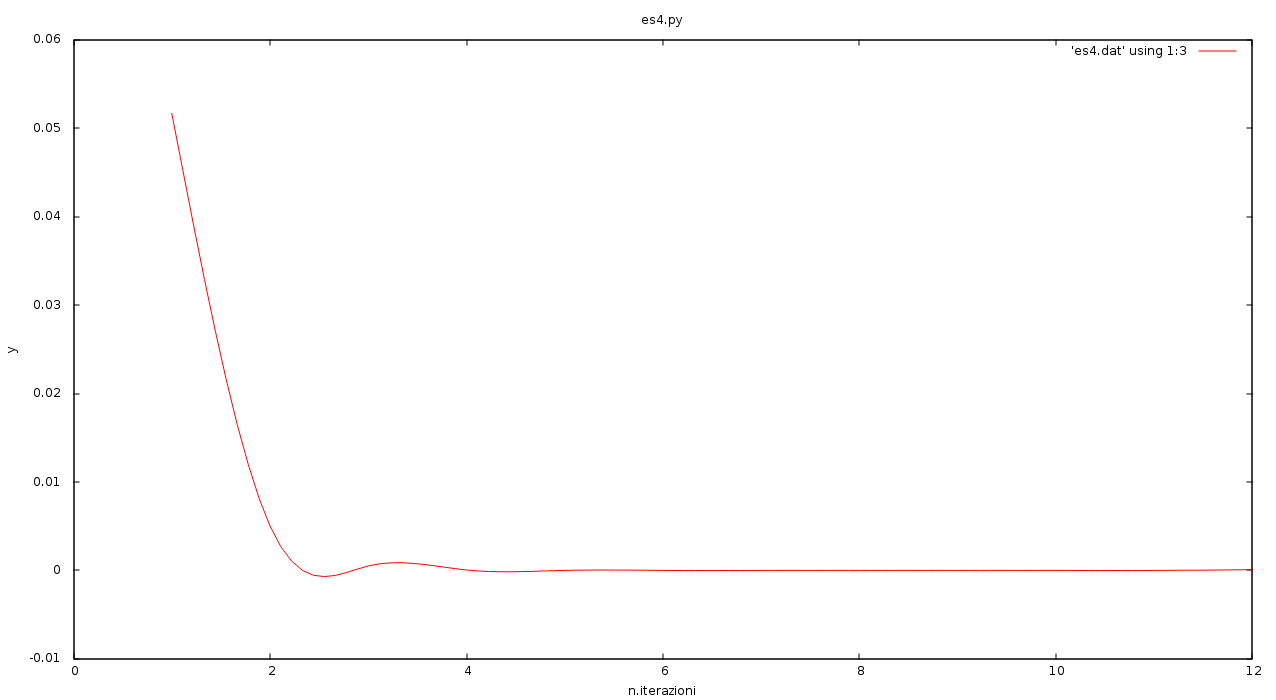
\includegraphics[width=\textwidth]{cap_1/es4/es4.png}

Si nota dal grafo come al crescere di i, quindi al diminuire di h, la precisione con cui viene approssimato f'(0) aumenta.
